% Source: graduate-coursework/Sp26/CSCE775/Project/proposal_asv_3/proposal3_asv.tex
% Description: System architecture. The SAC policy receives 87-dimensional observations from the ASV platform and its four heterogeneous sensors, outputs motion commands (heading, speed) and per-sensor duty-cycle ratios, and receives composite reward feedback from the water environment.

\documentclass[border=4pt]{standalone}
\usepackage{amsmath,amssymb}
\usepackage{pgfplots}
\usepackage{tikz}
\usepackage{xcolor}
\pgfplotsset{compat=1.18}
\usetikzlibrary{positioning, arrows.meta, shapes.geometric, fit, calc, backgrounds, patterns, decorations.pathreplacing}

\definecolor{Garnet}{HTML}{73000A}
\definecolor{Atlantic}{HTML}{466A9F}
\definecolor{Congaree}{HTML}{1F414D}
\definecolor{Horseshoe}{HTML}{65780B}
\definecolor{Rose}{HTML}{CC2E40}
\definecolor{Honeycomb}{HTML}{A49137}
\definecolor{Black90}{HTML}{363636}
\definecolor{Black70}{HTML}{5C5C5C}
\definecolor{Black50}{HTML}{A2A2A2}
\definecolor{Black30}{HTML}{C7C7C7}
\definecolor{Black10}{HTML}{ECECEC}
\definecolor{WarmGrey}{HTML}{676156}


\begin{document}
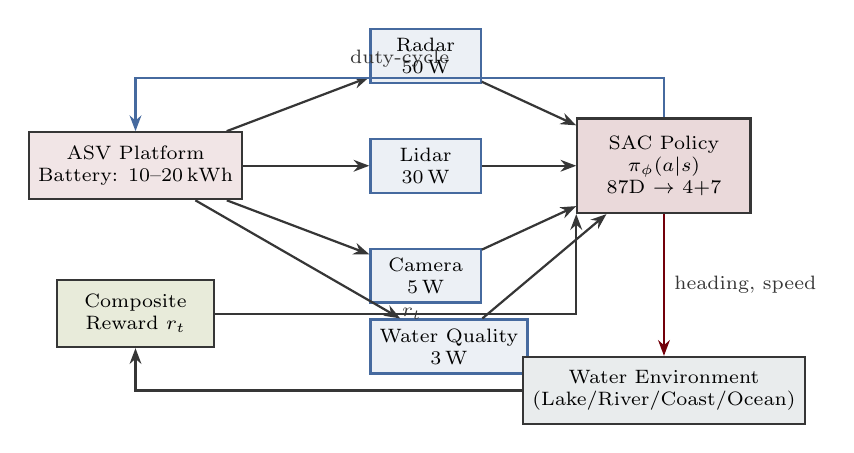
\begin{tikzpicture}[
    block/.style={draw=Black90, thick, minimum width=2.0cm, minimum height=0.85cm, align=center, font=\scriptsize},
    sensor/.style={draw=Atlantic, thick, minimum width=1.4cm, minimum height=0.6cm, align=center, font=\scriptsize, fill=Atlantic!10},
    arr/.style={-{Stealth[length=2mm]}, thick, color=Black90},
    every node/.style={font=\scriptsize}
]

% ASV Platform
\node[block, fill=Garnet!10, minimum width=2.4cm] (asv) {ASV Platform\\Battery: 10--20\,kWh};

% Sensors
\node[sensor, above right=0.6cm and 1.6cm of asv] (radar) {Radar\\50\,W};
\node[sensor, right=1.6cm of asv] (lidar) {Lidar\\30\,W};
\node[sensor, below right=0.6cm and 1.6cm of asv] (cam) {Camera\\5\,W};
\node[sensor, below right=1.5cm and 1.6cm of asv] (wq) {Water Quality\\3\,W};

% RL Policy
\node[block, fill=Garnet!15, right=1.2cm of lidar, minimum width=2.2cm, minimum height=1.2cm] (policy) {SAC Policy\\$\pi_\phi(a|s)$\\87D $\rightarrow$ 4+7};

% Environment
\node[block, fill=Congaree!10, below=1.8cm of policy, minimum width=2.6cm] (env) {Water Environment\\(Lake/River/Coast/Ocean)};

% Reward
\node[block, fill=Horseshoe!15, below=1.0cm of asv] (reward) {Composite\\Reward $r_t$};

% Arrows
\draw[arr] (asv) -- (radar);
\draw[arr] (asv) -- (lidar);
\draw[arr] (asv) -- (cam);
\draw[arr] (asv) -- (wq);
\draw[arr] (radar) -- (policy);
\draw[arr] (lidar) -- (policy);
\draw[arr] (cam) -- (policy);
\draw[arr] (wq) -- (policy);
\draw[arr, color=Garnet] (policy) -- node[right, color=Black90] {heading, speed} (env);
\draw[arr, color=Atlantic] (policy.north) -- ++(0,0.5) -| node[above, pos=0.25, color=Black90] {duty-cycle} (asv.north);
\draw[arr] (env) -| (reward);
\draw[arr] (reward) -| node[left, pos=0.3] {$r_t$} (policy.south west);

\end{tikzpicture}
\end{document}
